\chapter{LaRE - Laboratório Remoto Expansível}
\label{Capítulo3}
\begin{center}
    \textit{``All we have to decide is what to do with the time that is given us.''}

    Gandalf
\end{center}

Neste capítulo descreve-se o processo que levou à criação do \acrshort{lare}, a arquitectura de \textit{hardware} e \textit{software}, o motivo das escolhas e a implementação dos circuitos. \textbf{Acho que tem de ser refeito ou complementado}

\section{Contextualização}
\label{sec:contextualização}
Como já foi referido anteriormente (\textbf{ver a referência}) o principal objectivo desta dissertação passa pelo desenvolvimento de um \acrshort{laboratório remoto} para o ensino da electrónica, que visa colmatar (ou resolver) alguns dos problemas presentes no \acrshort{visir}.

Como referido na Secção \ref{sec:visir}, o \textit{software} do \acrshort{visir} foi lançado sob a licença GNU GPL. No entanto, o \textit{software} de programação do \textit{firmware} do controlador da matriz, que é vendido com a própria matriz, é proprietário da \acrshort{bth}. Quer isto dizer que não pode ser programado ou actualizado por terceiros. Ademais e como já foi referido na Secção \ref{sec:visir}, o equipamento que compreende módulos e placas de instrumentação são controlados pelo \acrshort{labview}, sendo que os preços das diversas versões variam, aproximadamente, entre os 523€ e os 4300€ anuais \cite{labviewpricing}.

A criação do \acrshort{laboratório remoto} surge como forma de resolver alguns dos problemas presentes no \acrshort{visir}.

Numa fase mais embrionária, foram feitos alguns testes de controlo de relés com o \gls{arduino} Mega, representado na Figura \ref{fig:arduinomega}, juntamente com um \acrfull{ide} simples desenvolvido em \acrshort{labview}.

\begin{figure}[hbtp]
    \centering
    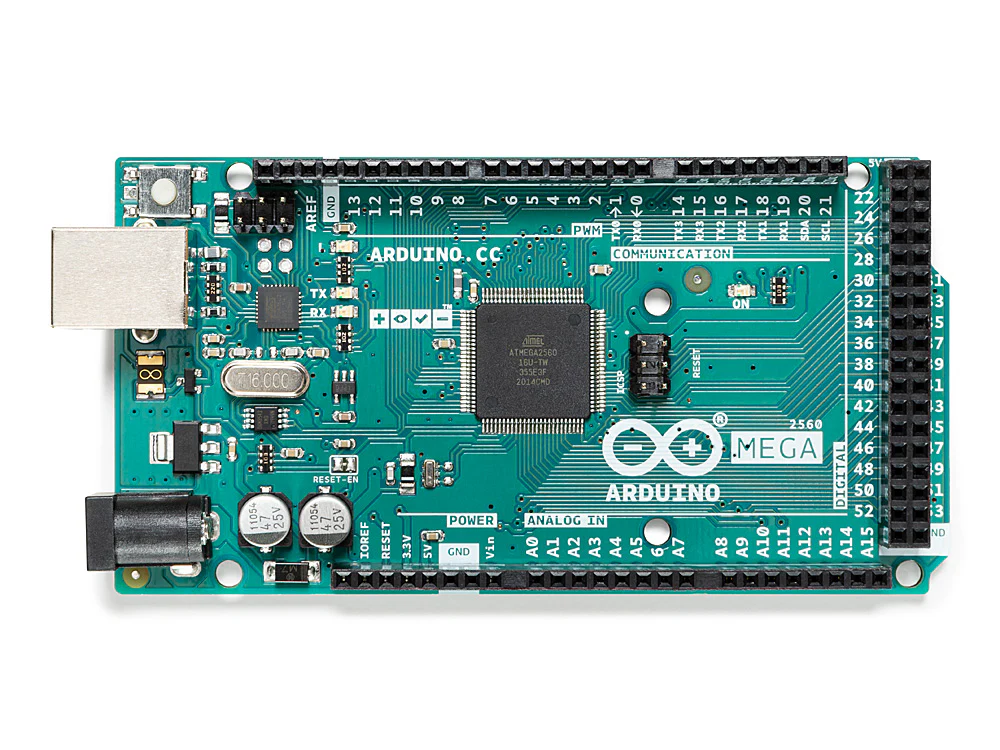
\includegraphics[width=0.6\textwidth]{figures/arduinomega.png}
    \caption{\textit{Arduino} Mega \cite{ArduinoMega}}
    \label{fig:arduinomega}
\end{figure}

No entanto, de forma a ultrapassar o problema levantado pelo elevado preço do \acrshort{labview}, surge um segundo objectivo que se prende com a substituição deste \textit{software}, por outro que fosse gratuito e \textit{open source}. A eliminação do \acrshort{labview} implicou a implementação de um servidor. Sendo assim, e numa primeira abordagem, foram analisadas algumas opções. Tais como: \textit{FastApi}\footnote{\url{https://fastapi.tiangolo.com/}}, \textit{Django}\footnote{\url{https://www.djangoproject.com/}} e \textit{Flask}\footnote{\url{https://flask.palletsprojects.com/en/3.0.x/}}.

As opções analisadas enquadram-se no que se pode chamar \textit{frameworks} ou \textit{micro-frameworks}. Neste caso são todas desenvolvidas para aplicação em \gls{python}.

Uma \textit{micro-framework} é um tipo de \textit{framework} minimalista, que fornece apenas as funcionalidades essenciais para o desenvolvimento de aplicações, sem incluir bibliotecas ou componentes adicionais que não as estritamente necessárias. Isso permite a quem desenvolve adicionar apenas as funcionalidades especificas a cada projecto ou aplicação. Daqui resulta um ambiente de desenvolvimento mais leve e flexível \cite{Flask}.
Optou-se, então, pelo \textit{Flask} e as razões da escolha, assim como uma explicação mais detalhada serão apresentadas na Secção \ref{sec:software}.

É possível combinar o \gls{arduino} com o \gls{python}, mas isso implicaria uma mudança ao nível do \textit{firmware}, uma tarefa que não é de forma alguma, trivial \cite{Arduinopython}. A linguagem nativa do \gls{arduino} é similar ao C++ e o \textit{firmware} instalado foi projectado para interpretar e executar código escrito nesse tipo de linguagem. Para seremos mais rigorosos, o uso do \textit{Python} no \gls{arduino} ou em qualquer outro microcontrolador, faz-se através de \textit{MicroPython}, uma implementação simples e eficiente do \gls{python} que inclui um pequeno subconjunto da bibliotecas padrão e é optimizado para funcionar em microcontroladores e em ambientes limitados \cite{MicroPythondefinition}. Quer isto dizer que, todas as bibliotecas usadas na programação da aplicação ou projecto têm de ser carregadas para a memória dos microcontroladores. No caso do \gls{arduino} Mega, uma análise ao \textit{datasheet} \cite{megadatasheet} revela que este possuiu \SI{256}{Kbytes} reservados para o envio de programas e \SI{8}{Kbytes} de memória \textit{SRAM}, reservada para variáveis temporárias.
Além destes problemas de memória apresentados, e uma vez que é necessário que o \gls{arduino} funcione como servidor, a versão apresentada na Figura \ref{fig:arduinomega} não é adequada.

No mercado, existe o \gls{ESP32}, uma alternativa mais poderosa que o \gls{arduino} e com placa de rede sem fios integrada, tal como apresentado na Figura \ref{fig:ESP32}. No entanto, este microcontrolador sofre dos mesmos problemas de memória que o \gls{arduino} Mega e da utilização do \textit{MicroPython}. Uma análise ao \textit{datasheet} \cite{esp32datasheet} revela que, a memória \textit{flash} varia entre os 4-16 \acrlong{mb}. No modelo ''ESP32-DEVKITC-32E``, que estava disponível para este projecto, o valor é de 4 \acrshort{mb} \cite{diferencaspython}.

Estas limitações não permitem a implementação de um servidor minimamente robusto usando o \gls{arduino} Mega ou o \gls{ESP32}.

\begin{figure}[hbtp]
    \centering
    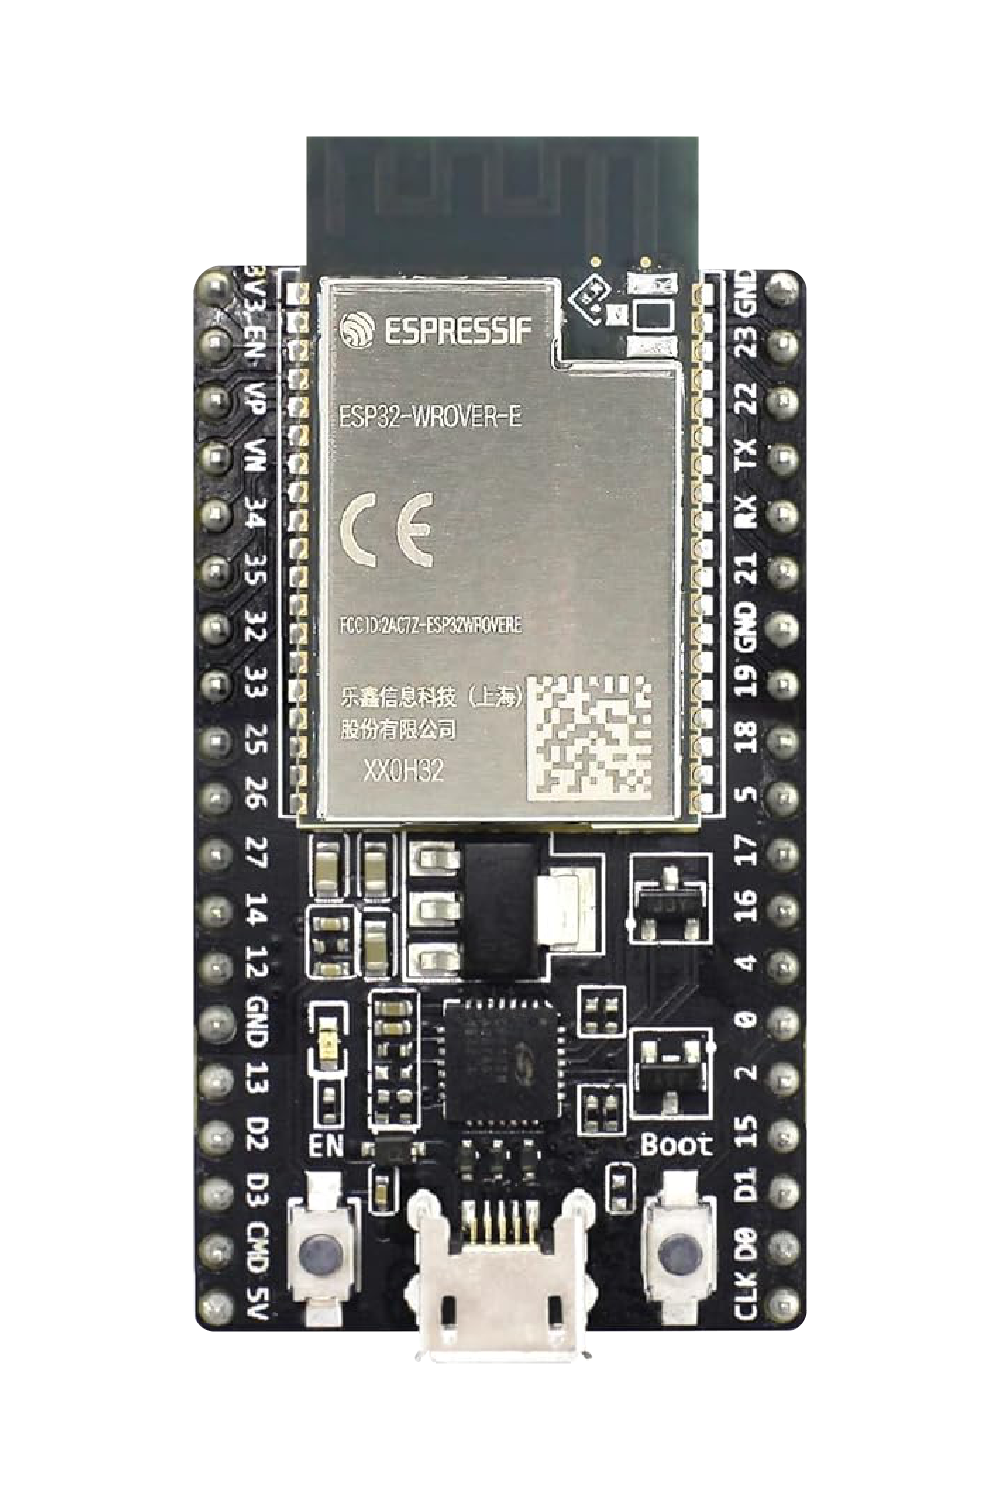
\includegraphics[width=0.4\textwidth]{figures/ESP32-DevKitC_L_0.png}
    \caption{\textit{ESP32} \cite{ESPDevKit}}
    \label{fig:ESP32}
\end{figure}

A escolha seguinte recaiu no \gls{RaspberryPI}, versão 5, apresentada na Figura \ref{fig:Raspberrypi5}. Este dispositivo insere-se numa gama de pequenos computadores, acessíveis e versáteis que podem ser utilizados para os mais variados projectos. Na Secção \ref{sec:hardware} apresenta-se uma descrição mais detalhada do \gls{RaspberryPI}.

\begin{figure}[hbtp]
    \centering
    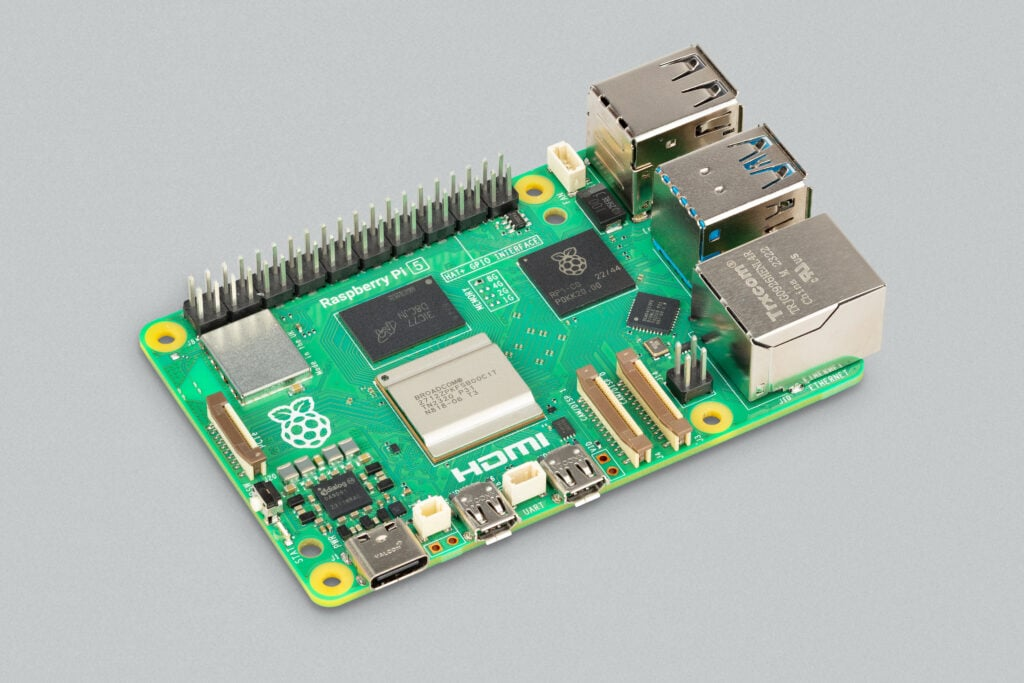
\includegraphics[width=0.6\textwidth]{figures/raspberrypi5.jpg}
    \caption{\textit{RaspberryPI5} \cite{introRaspberrypi5}}
    \label{fig:Raspberrypi5}
\end{figure}

Considerou-se, portanto, que seria uma mais-valia desenvolver um \acrshort{laboratório remoto} com as seguintes características:
\begin{itemize}
    \item \gls{python} como linguagem principal;
    \item \gls{RaspberryPI} como servidor \textit{Flask};
    \item \textit{Interface} com o utilizador desenvolvido em \acrshort{html}.
\end{itemize}

Estava dado o passo final para o que viria a ser o \acrshort{lare}.

\section{Solução proposta}
\label{sec:solucaoproposta}
Os objectivos principais foram definidos na Secção \ref{sec: Objectivos} e as características gerais definidas na Secção \ref{sec:contextualização}.

Pretende-se que o \acrshort{lare} seja um \acrshort{laboratório remoto} capaz de controlar e comandar um conjunto de experiências electrónicas, assim como efectuar medições de várias grandezas electricas. Para que a solução proposta fique completa e definitiva, falta definir os instrumentos de medida, assim como os circuitos que compõem as experiências.

No contexto desta dissertação, o instrumento de medida sugerido para implementar o \acrshort{lare} foi o \textit{VirtualBench}, modelo VB-8012.

O \textit{VirtualBench} pode ser controlado de duas formas: através do \textit{software} fornecido pela \acrshort{ni} ou através do \textit{pyVirtualBench} \cite{AutomatingVB}.

O \textit{pyVirtualBench} é um \gls{wrapper}\footnote{Este \gls{wrapper} é um \textit{software} de terceiros, suportado e mantido pela comunidade e não é diretamente suportado pela \acrshort{ni}.} que permite controlar o \acrshort{virtualbench} através de uma aplicação \gls{python} \cite{pyvirtualbench}. No entanto, este \gls{wrapper} não é compatível com \textit{Linux}.
Perante este facto, decidiu-se integrar um \acrshort{pc} no \acrshort{lare} - pormenores da instalação do \textit{driver} no \textit{site} da \acrshort{ni} (\href{https://knowledge.ni.com/KnowledgeArticleDetails?id=kA00Z000000kHUFSA2&l=pt-PT}{\textit{link}}) - sendo que todo o peso computacional passaria para o \acrshort{pc} e o \gls{RaspberryPI} controlaria os relés. Esta decisão de o manter como controlador dos relés prendeu-se com o facto de, futuramente, poder haver espaço para uma evolução ao nível da compatibilidade com o \textit{pyVirtualBench}.

A outra forma de controlar o \acrshort{virtualbench} é usando a aplicação disponibilizada pela \acrshort{ni}  e compatível com \textit{Windows}. Esta aplicação faz uma apresentação integrada dos cinco instrumentos apresentados no \acrshort{virtualbench}, como pode ser visto na Figura \ref{fig:leituraohm}. A aplicação também inclui funcionalidades de fluxo de trabalho, como a importação e exportação de configurações de instrumentos e a captura de dados\footnote{\href{https://www.ni.com/en/support/downloads/drivers/download.virtualbench-software.html}{Transferir VirtualBench}}.

De referir que o \acrshort{virtualbench} não pode ser controlado pelo \textit{pyVirtualBench} e pelo \textit{software} simultaneamente.

\begin{figure}[hbtp]
    \centering
    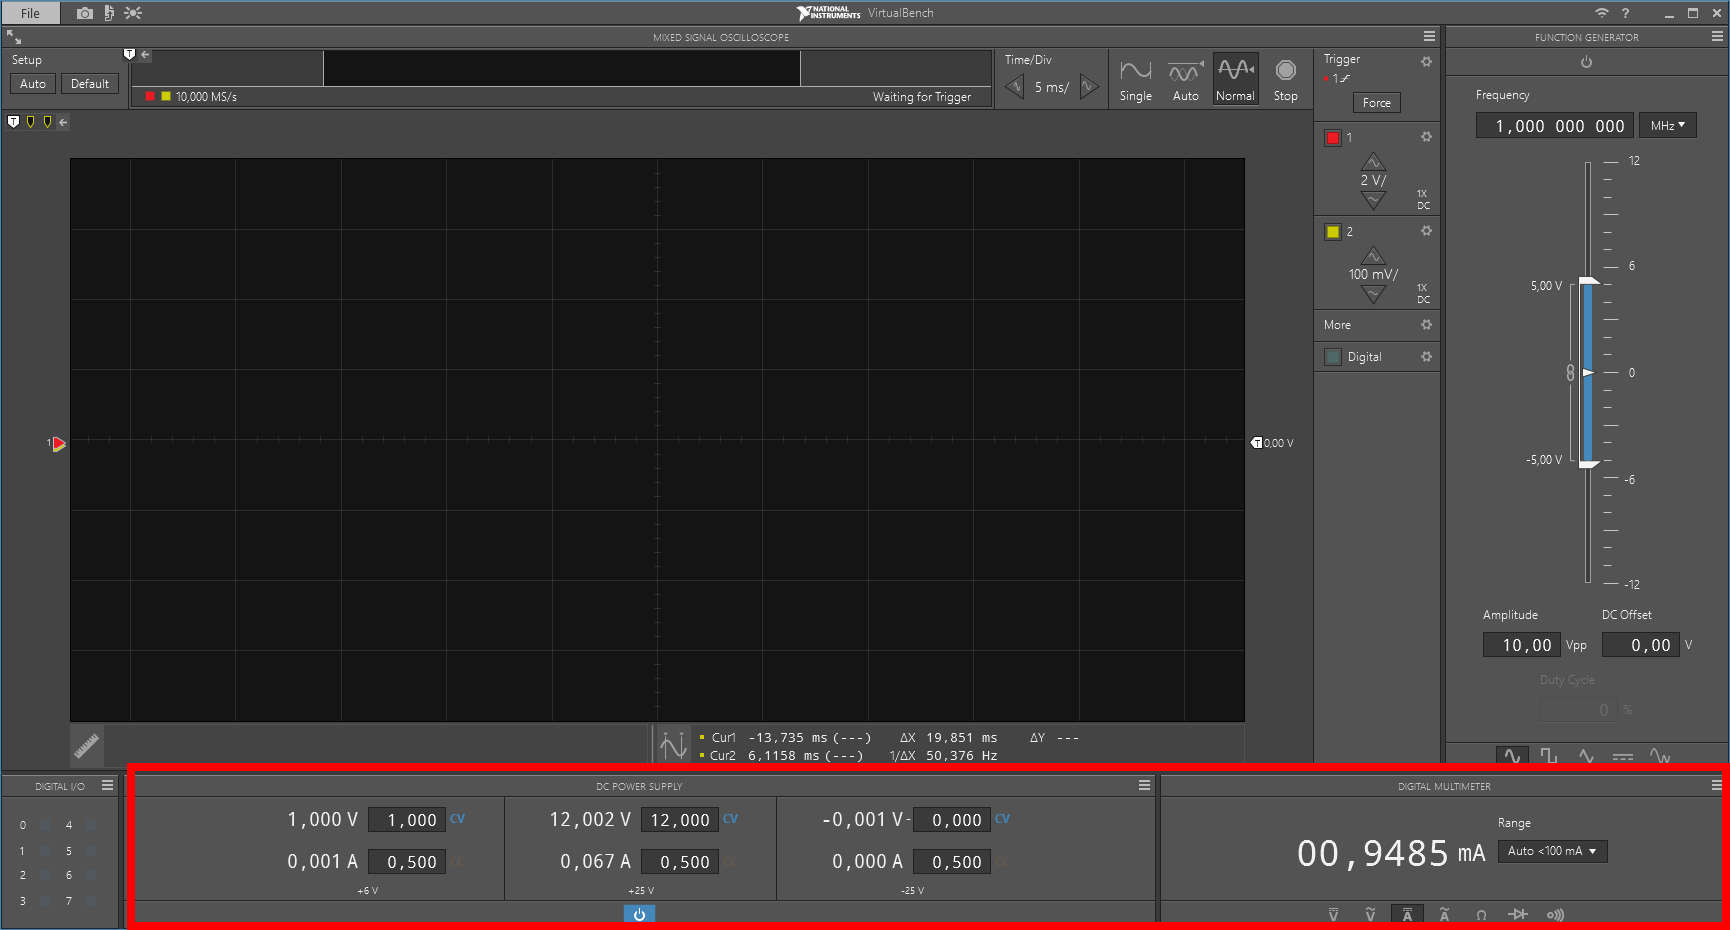
\includegraphics[width=0.9\textwidth]{figures/VB8012-OHM_Exemplo.png}
    \caption{Exemplo do \acrshort{virtualbench} usado como multímetro digital}
    \label{fig:leituraohm}
\end{figure}

As características do \acrshort{laboratório remoto} são, agora, as seguintes:
\begin{itemize}
    \item \gls{python} como linguagem principal;
    \item \acrshort{pc} como servidor \textit{Flask};
    \item \gls{RaspberryPI} como controlador dos relés;
    \item \textit{Interface} com o utilizador desenvolvido em \acrshort{html}.
\end{itemize}

Definidas - de uma forma geral - as soluções de \textit{hardware} e \textit{software}, agora com a integração de um \acrshort{pc} - passou-se ao estudo da arquitectura do \acrshort{lare}.

\section{Arquitectura}
\label{sec:arquitectura}
Como já se viu na Secção \ref{sec:contextualização} a arquitectura do \acrshort{lare} proposta baseia-se numa estrutura cliente-servidor, suportada ao nível do \textit{hardware} pelo \acrshort{virtualbench}, pelo \gls{RaspberryPI} e um \acrshort{pc} como servidor. Uma representção geral do que será o \acrshort{lare} pode ser vista na Figura \ref{fig:representaçãogerallare}.

\begin{figure}[hbtp]
    \centering
    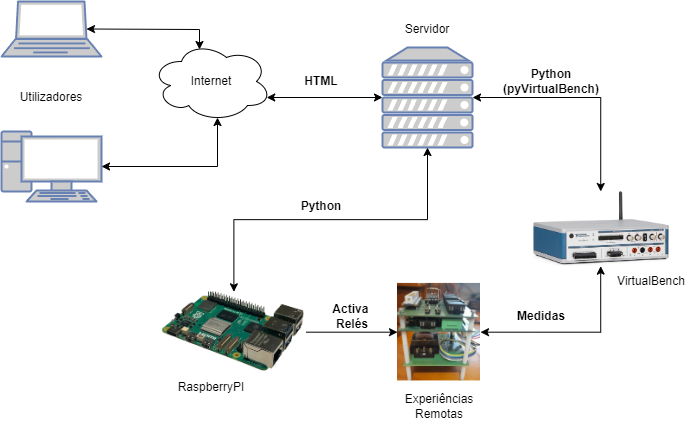
\includegraphics[width=1\textwidth]{figures/arquitectura_ver2.drawio.png}
    \caption{Representação geral do \acrshort{lare}}
    \label{fig:representaçãogerallare}
\end{figure}

Antes de mais, importa clarificar as formas de comunicação entre os diversos dispositvos que compõem o \acrshort{lare}. Tanto o servidor, como o \gls{RaspberryPI} e o \acrshort{virtualbench} têm disponíveis interfaces de rede sem fios e com fios, assim como \textit{interfaces} \acrshort{usb}.

A comunicação entre os diversos dispositivos é feito da seguinte forma:
\begin{itemize}
    \item \textbf{Servidor - \gls{RaspberryPI}}: comunicação via rede sem fios. Em termos de simplicidade de programação, a comunicação entre o servidor e o \gls{RaspberryPI} é feita através da rede sem fios, utilizando \textit{sockets}. Os \textit{sockets} e a \acrshort{api} de \textit{sockets} facilitam a comunicação entre processos em redes, quer estas sejam físicas (ligadas a outras através de fios ou sem fios) ou lógicas (como a rede local de um computador). Isto é, permitem o envio de mensagens através de uma rede \cite{Sockets};
    \item \textbf{Servidor - \acrshort{virtualbench}}: comunicação via rede sem fios ou \acrshort{usb}. Entre estes dois dispositivos é, basicamente, indiferente a forma como é feita a comunicação. Isto porque esta parte é gerida pelos \textit{drivers} da aplicação instalada no \textit{Windows}. Independentemente de se utilizar o \textit{pyVirtualBench} ou a aplicação.
    \item \textbf{Controlo de relés e medidas}: O controlo e medição comum às experiência é feito através de ligações directas aos dispositivos.
\end{itemize}

Ao nível do \textit{software}, o servidor será implementado com base no \textit{Flask}, como já foi referido na Secção \ref{sec:contextualização} e será descrito com mais pormenor na Secção \ref{sec:software}. A comunicação entre o servidor e o \acrshort{virtualbench}, entre o servidor e o \gls{RaspberryPI} e o controlo dos relés é feita em \textit{Python}. A \textit{interface} com o utilizador é feita em \acrshort{html}.

A Figura {\ref{fig:arquitecturalore}} apresenta com mais pormenor a solução implementada no \acrshort{lare}. De uma forma geral, podemos ver como é realizada a comunicação e a troca de informação entre os diferentes dispositivos de \textit{hardware}.

\begin{figure}[hbtp]
    \centering
    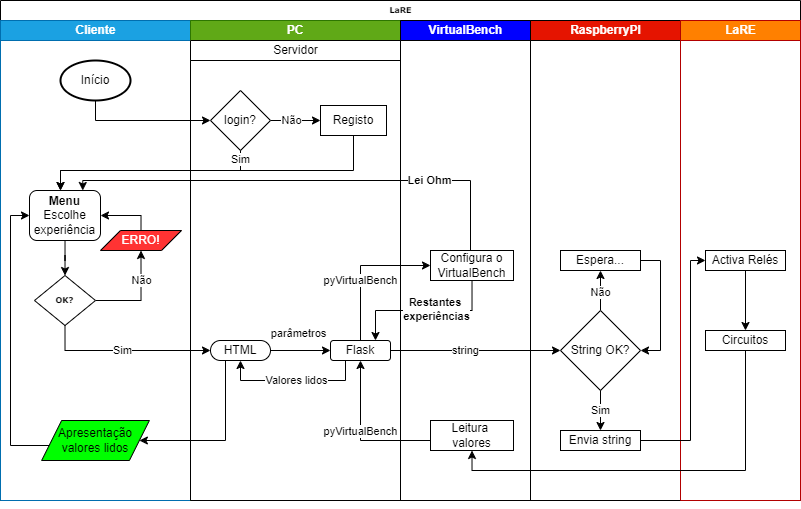
\includegraphics[width=1\textwidth]{figures/Diagrama_SOFTWARE.drawio.png}
    \caption{Arquitectura \acrshort{lare}}
    \label{fig:arquitecturalore}
\end{figure}

\section{Circuitos electrónicos - experiências?}
\label{sec:circuitos}
\textbf{Não sei até que ponto esta secaçõp não se enquadra melhor no hardware}
A escolha dos circuitos teve como base os que estão disponíveis no \acrshort{visir} do \acrshort{isep}, como se pode ver na Figura \ref{fig:circuitosvisir}. Reduzindo os objectivos do \acrshort{lare} à sua forma mais básica, pode afirmar-se que se pretende ``provar um conceito''. Escolhendo experiências com circuitos integrados ou transístores, poderia tornar a implementação desnecessáriamente mais complexa e, por conseguinte, com menos experiências. Portanto, o objectivo passará por criar um \acrshort{laboratório remoto} com experiências típicas para a introdução à electrónica e que permitam uma aprendizagem gradual em contexto de sala de aula. E, assim, ``provar o conceito''.

\begin{figure}[hbtp]
    \centering
    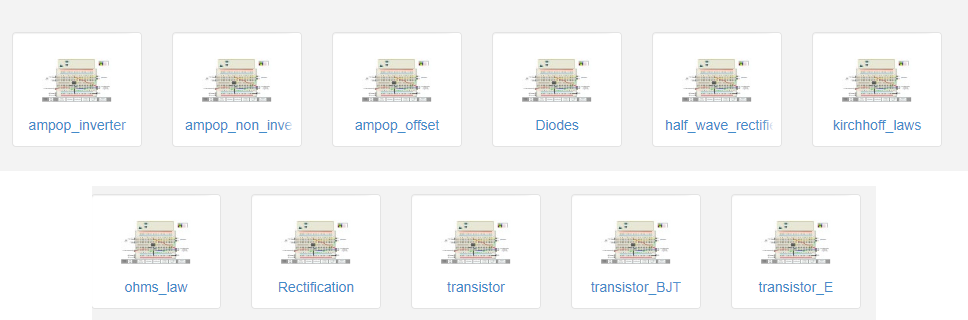
\includegraphics[width=1\textwidth]{figures/visir_ISEP.png}
    \caption{Circuitos \acrshort{visir} - \acrshort{isep} - \textbf{Se calhar retirava a imagem}}
    \label{fig:circuitosvisir}
\end{figure}

Sendo assim, os circuitos que compõem o \acrshort{lare} e satisfazem os critérios definidos em cima são:
\begin{itemize}
    \item Lei de Ohm;
    \item Rectificador de meia onda;
    \item Rectificador de onda completa;
    \item Filtro RC passa-baixo;
    \item Filtro RC passa-alto.
\end{itemize}

\section{Hardware}
\label{sec:hardware}
\subsection{VirtualBench}
Este dispositivo desenvolvido pela \acrshort{ni} integra vários instrumentos e ferramentas de teste, tais como um osciloscópio digital com análise de protocolo, um gerador de formas de onda, um multímetro digital, uma fonte de alimentação \acrfull{cc} programável e E/S digitais num único dispositivo que se liga a um \acrshort{pc}, via \acrshort{usb} ou rede sem fios, como se pode ver na Figura \ref{fig:paineltraseiro}. As principais características deste modelo estão descritas na Figura \ref{fig:paineldianteiro} \cite{datasheetVirtualBench}. A forma como pode ser controlado e configurado já foi abordada na Secção \ref{sec:arquitectura}.

\begin{figure}[hbtp]
    \centering
    \centering
    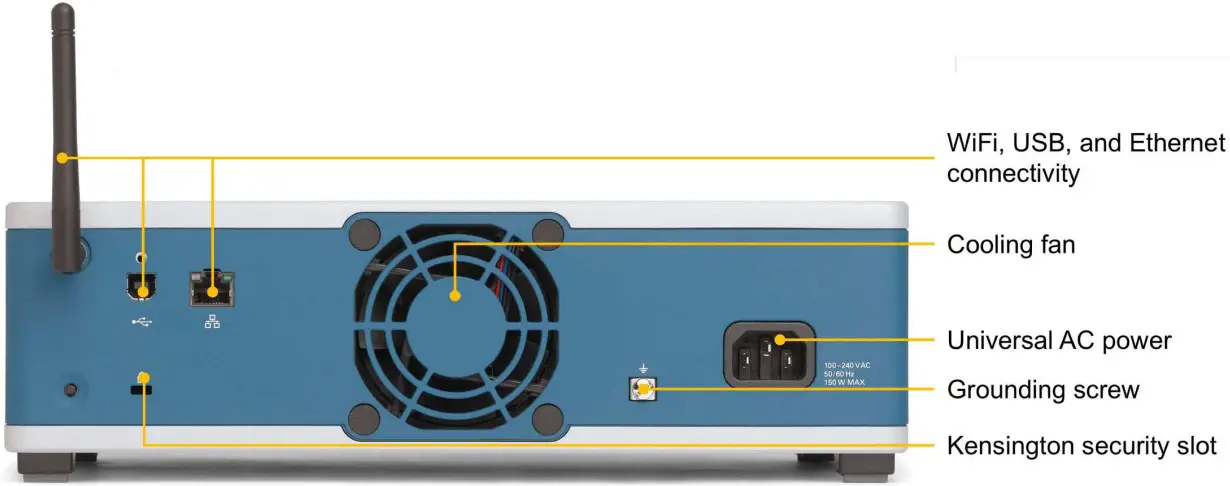
\includegraphics[width=0.9\textwidth]{figures/virtualbench_back-panel.jpg}
    \caption{Painel traseiro \textit{VirtualBench} VB-8012  \cite{datasheetVirtualBench}.}
    \label{fig:paineltraseiro}
\end{figure}

\begin{figure}[hbtp]
    \centering
    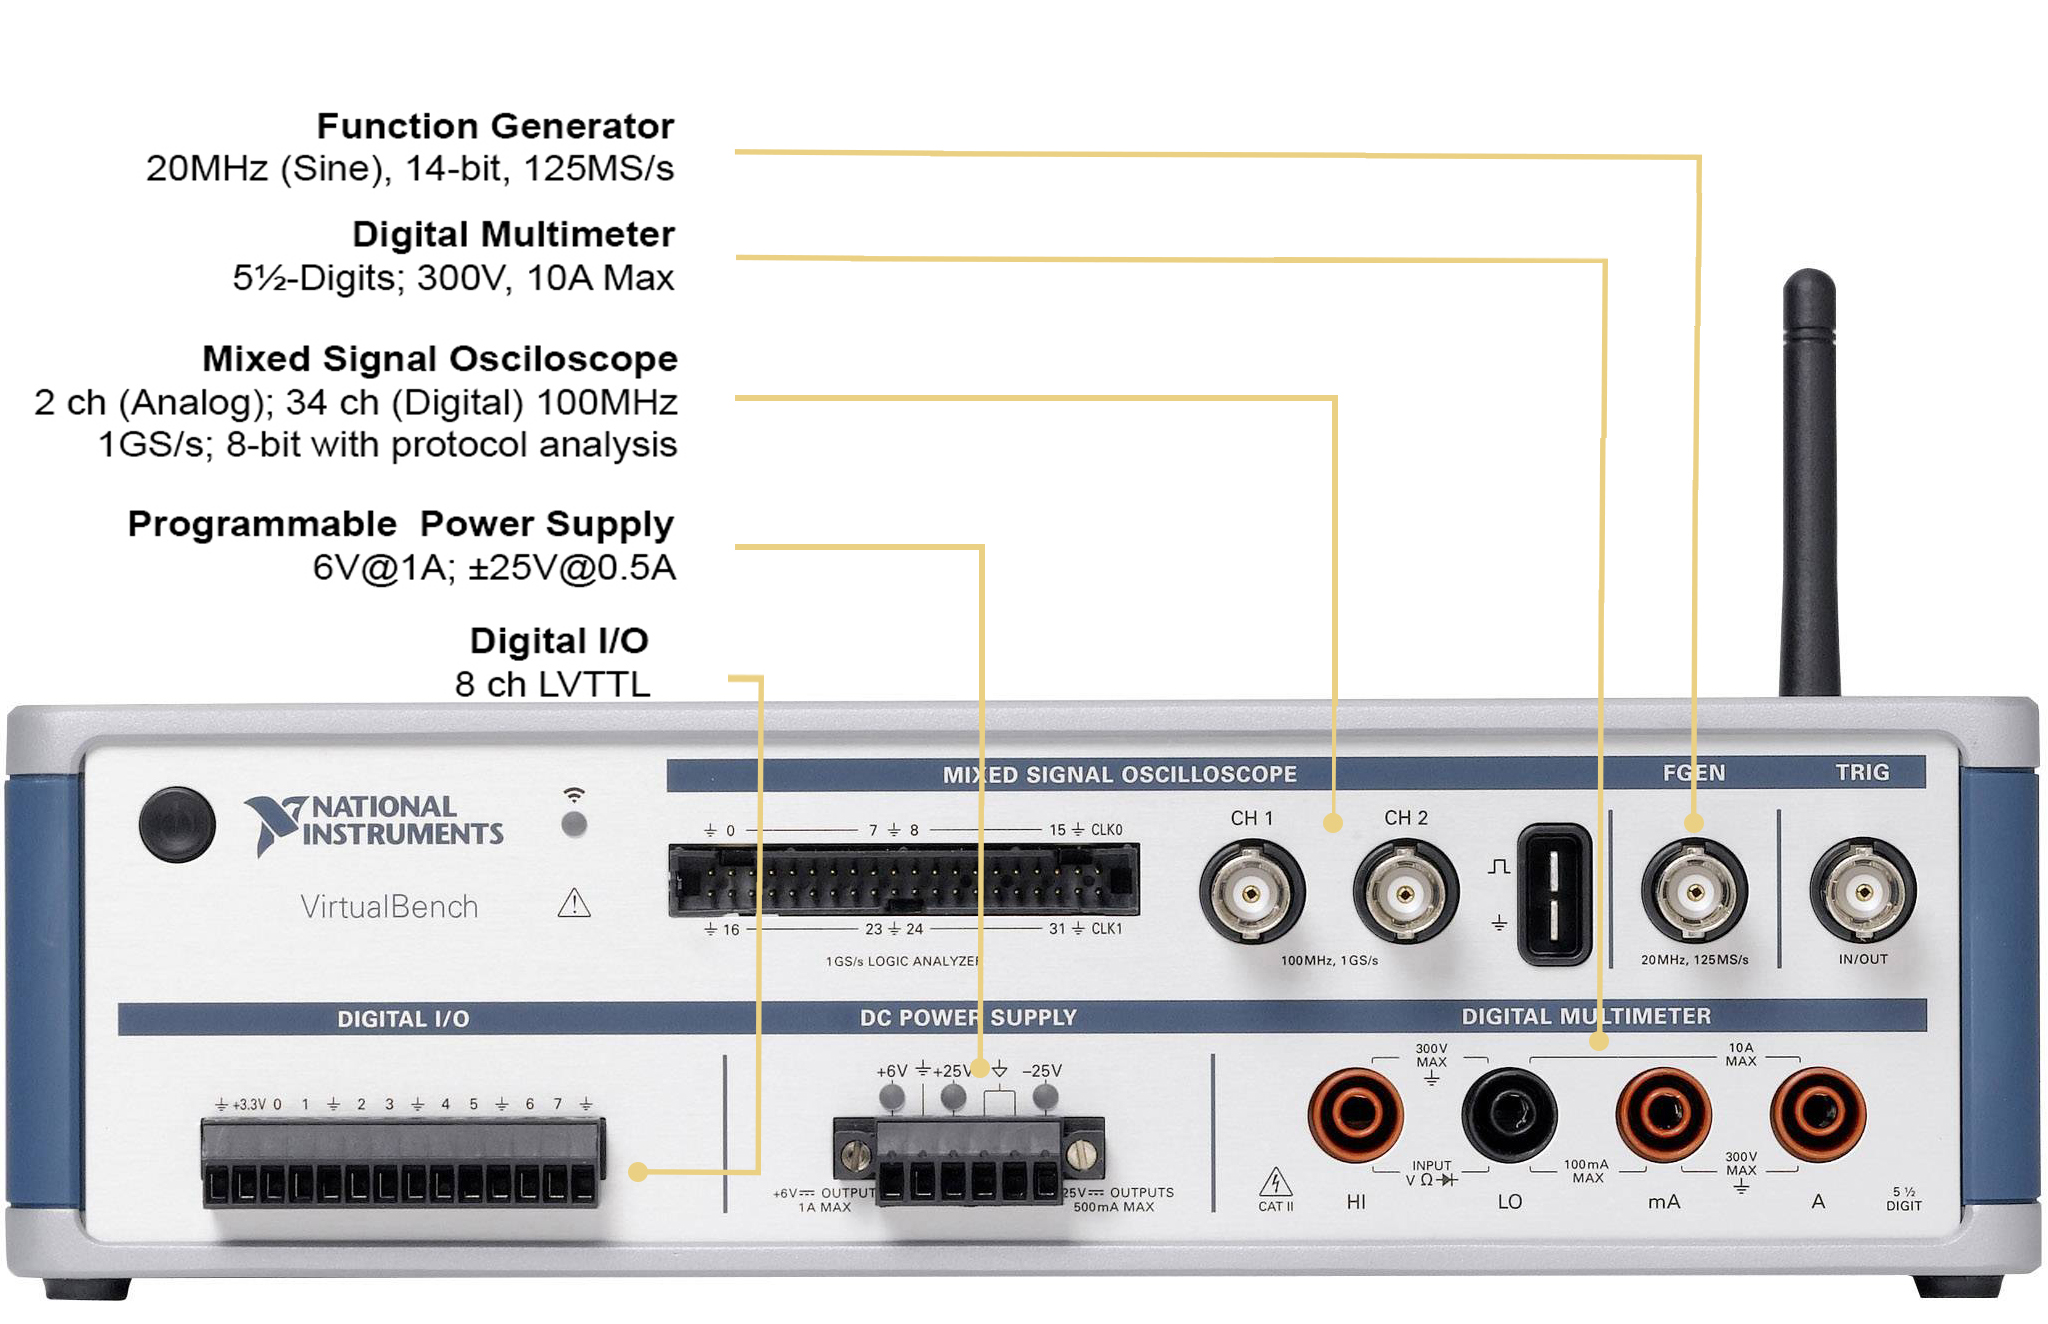
\includegraphics[width=0.9\textwidth]{figures/virtualbench_front-panel.jpg}
    \caption{Painel frontal \textit{VirtualBench} VB-8012  \cite{datasheetVirtualBench}.}
    \label{fig:paineldianteiro}
\end{figure}

%No \acrshort{visir} do \acrshort{isep}, estão disponíveis 11 circuitos, como se pode ver na Figura \ref{fig:circuitosvisir}. Os circuitos que compõem o \acrshort{laboratório remoto} tiveram como base (ou ponto de partida) os que estão implementados no \acrshort{isep}. \textbf{Faz sentido? PROF}


\subsection{Matriz LaRE}
Encontradas as soluções de \textit{hardware} e \textit{software}, assim como as experiências a serem implementadas, partiu-se para o projecto dos circuitos.

Mais uma vez, tomando como base o \acrshort{visir}, decidiu-se projectar uma matriz com a dimensão das placas a obedecerem às definidas pela consórcio \gls{pc/104} \cite{PC104}. Este consórcio definiu um padrão que se destaca pelo seu formato compacto e modular. As dimensões mecânicas das placas estão definidas no \textbf{referência ao datasheet}.

Esta matriz, que inclui os circuitos definidos na Secção \ref{sec:solucaoproposta}, assim como a alimentação e as ligações ao \gls{RaspberryPI}, compõe as 5 experiências.

Esta matriz é composta por 3 placas:
\begin{itemize}
    \item Alimentação:
          \begin{itemize}
              \item Transformador;
              \item Fonte de tensão de \SI{5}{\volt};
          \end{itemize}
    \item Circuito da Lei de Ohm;
    \item Circuitos de Rectificação e filtros:
          \begin{itemize}
              \item Rectificação de meia onda;
              \item Rectificação de onda completa;
              \item Filtro passa-baixo;
              \item filtro passa-alto.
          \end{itemize}
\end{itemize}



Toda a informação relevante referente à Matriz encontra-se no \textit{datasheet} em anexo. [\textbf{Confirmar as referências e local da aprsentação do datasheet}]

\subsection{Objectivos}
\subsection{Análise de alternativas/razões das opções}
\textbf{Eventualmente já foram abordadas as escolhas do software e hardware no contexto}


\subsection{RaspberryPI}
Como já foi referido na Secção \ref{sec:contextualização}, a ideia inicial passava por utilizar o \gls{RaspberryPI} como servidor e como controlador dos relés, no fundo desempenhando as funções de \acrshort{rlms}.

Em contexto de laboratório estavam disponíveis os modelos PI2 e PI3, algo desactualizados. O PI3 já se mostrou lento nos primeiros testes e, por isso, optou-se pela última versão do \textit{RaspberryPI}\footnote{Doravante, sempre que for referido \textit{RaspberryPI}, subentende-se a versão 5.}.

As principais diferenças de \textit{hardware} entre a versão 5 e a 4B estão representadas na Tabela \ref{Table:diferencasPI4PI5}. Estas melhorias acarretam um maior consumo de energia e, por isso, é recomendado o uso de arrefecimento. Na Figura \ref{fig:pi5dissipador} está representado o \gls{RaspberryPI} usado no \acrshort{lare}.

\textbf{Referência aos pinos no datasheet?}

\begin{figure}[hbtp]
    \centering
    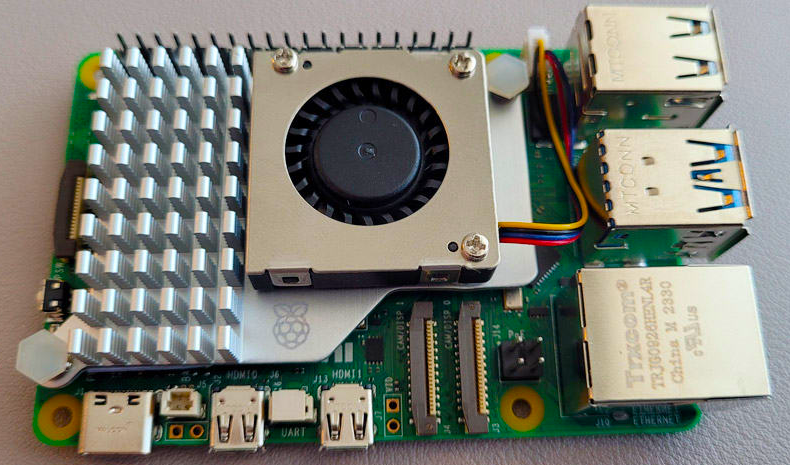
\includegraphics[width=1\textwidth]{figures/pi5_dissipador.png}
    \caption{\textit{Raspberry PI5} com dissipador activo utilizado no \acrshort{lare}}
    \label{fig:pi5dissipador}
\end{figure}

\begin{table}[htb]
    \centering
    \caption{Raspberry PI4 \textit{vs Raspberry PI5 - principais diferenças} \cite{Raspberrypi5}}
    \label{Table:diferencasPI4PI5}
    \begin{tabular}{ll}
        \toprule
        Raspberry PI4                                            & Raspberry PI5                                             \\
        \midrule
        \SI{1.8}{\giga\hertz}                                    & \SI{2.4}{\giga\hertz}                                     \\
        \midrule
        VideoCore VI @ \SI{500}{\mega\hertz}, Vulkan 1.0         & VideoCore VII @ \SI{800}{\mega\hertz}, Vulkan 1.2         \\
        \midrule
        LPDDR4-3200 SDRAM até \SI{8}{\giga\byte}                 & LPDDR4X-4267 SDRAM \SI{4}{\giga\byte}/\SI{8}{\giga\hertz} \\
        \midrule
        \SI{5}{\volt}/\SI{3}{\ampere} via USB-C (\SI{15}{\watt}) & \SI{5}{\volt}/\SI{5}{\ampere} via USB-C (\SI{27}{\watt})  \\
        \bottomrule
    \end{tabular}
\end{table}

\subsection{Relés}
Os relés utilizados estavam disponíveis em contexto laboratorial e são em tudo idênticos aos que se encontram montados no \acrshort{visir}  do \acrshort{isep}.

No \acrshort{lare} foram usados dois tipos de relés - simples, \acrfull{spst} e duplos, \acrfull{dpst}, como se pode ver na Figura \ref {fig:reles}.

Os modelos utilizados foram ambos da \textit{Comus}: relé \acrshort{spst}, ref. 3570-1331-123 e relé \acrshort{dpst}, ref. 3572-1220-123. As características mais importantes encontram-se descritas no \textit{datasheet} anexo a este documento. \textbf{Ver a referência ao datasheet}. Os dois primeiros quartetos indicam a série do relé e os três números indicam a tensão da bobine e a presença, ou não, do díodo de ``roda livre''. No caso dos relés usados, a tensão da bobine é de \SI{12}{\volt} e o díodo está ligado entre os pinos 2(+) e 6(-) \cite{DryRelay}. Tentou-se, sempre que possível, utilizar os relés \acrshort{spst} no comando das fontes e aparelhos de medida e os relés \acrshort{dpst} no controlo dos componentes. Serão devidamente referidos os casos em que isso não foi possível, por indisponibilidade dos componentes.

\begin{figure}[hbtp]
    \centering
    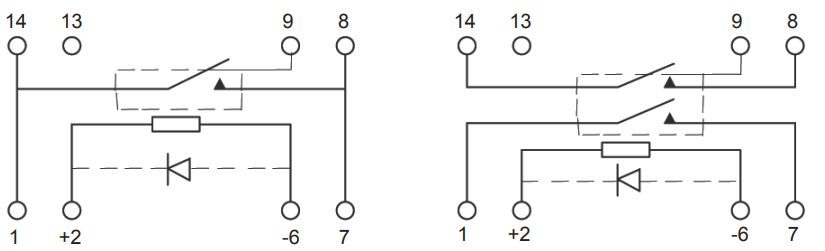
\includegraphics[width=1\textwidth]{figures/reles.png}
    \caption{\textit{Relés \acrshort{spst} e \acrshort{dpst}} \cite{DryRelay}}
    \label{fig:reles}
\end{figure}

Segundo a informação técnica disponibilizada em \cite{Raspberrytech}, a tensão de funcionamento dos \acrfull{gpio}s, quer estejam configurados como entrada ou saída, é de \SI{3.3}{\volt}, sendo que a máxima corrente por cada \acrshort{gpio} é de \SI{16}{\mA}. No caso extremo de todas os 17 \acrshort{gpio}s estarem activos ao mesmo tempo, a corrente total seria de \SI{272}{\mA}. Nesta situação, a fonte de \SI{3.3}{\volt} colapsava.
Por isso, para que o RaspberryPI possa comandar os relés com segurança, é necessário o uso de \textit{drivers} que consigam fornecer a tensão e corrente necessária para o efeito.

\subsection{\textit{Driver} de Relés}
O circuito integrado ULN2003A é um \textit{driver} muito usado para controlar relés. Além disso e mais uma vez, estava disponível em contexto laboratorial.
Tipicamente, este \textit{driver} é usado em conjunto com micro-controladores ou \gls{RaspberryPI} no comando de cargas indutivas, como motores, bobines e relés.

Os ULN2003A possuem sete pares de transístores NPN, em configuração \textit{Darlington}, que apresentam saídas de alta tensão com díodos \textit{clamp} de cátodo comum para comutação de cargas indutivas \cite{ULN2003}, como se  representa esquematicamente na Figura \ref{fig:2003blocos}.

\begin{figure}[hbtp]
    \centering
    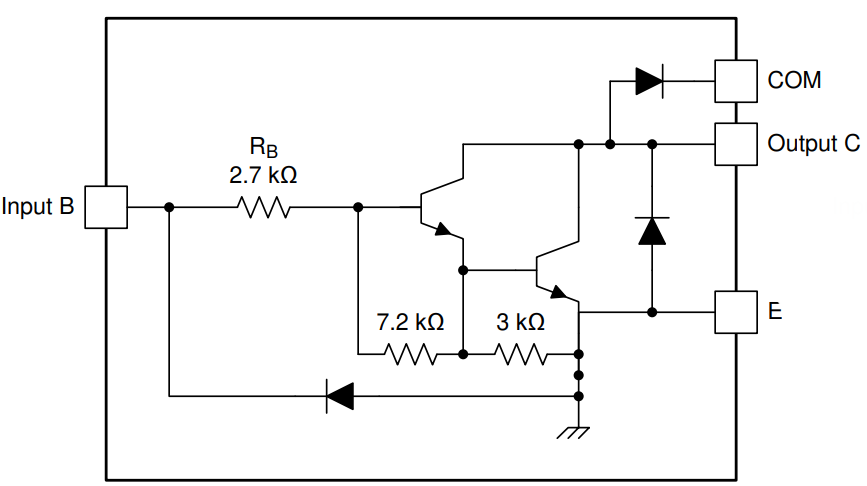
\includegraphics[width=1\textwidth]{figures/2003A_Darling.png}
    \caption{Diagrama de blocos ULN2003A \cite{ULN2003}}
    \label{fig:2003blocos}
\end{figure}

A corrente de colector de saída (única) é de \SI{500}{\mA} e a corrente de entrada, para uma tensão de entrada de \SI{3.85}{\volt}, é \SI{0.93}{\mA} \cite{ULN2003}.

Pela análise dos esquemas \textbf{DATASHEET - REFERÊNCIA} verifica-se que os \acrshort{gpio}s disponíveis no \gls{RaspberryPI} - 17 no total - não são suficientes para comandar os relés do \acrshort{lare}. Ao todo são utilizados 21 relés, o que corresponderia a 21 saídas. A placa correspondente à experiência da Lei de Ohm, possui 8 relés. No caso da placa correspondente às experiências dos circuitos de rectificadores e filtros, o número de relés para efectuar as experiências é de 13. Falta adicionar os 10 \acrshort{gpio}s necessários para o controlo da transmissão das tramas de \textit{bits} \footnote{Este procedimento será abordado com mais \textbf{rigor, explicado melhor, blá, blá, nas secções seguintes - COLOCAR REFERÊNCIA}}.

Sendo assim, houve a necessidade de criar uma solução que permitisse comandar os relés, já que o \gls{RaspberryPI} não possui \acrshort{gpio}s suficientes.

\subsection{Registo de deslocamento}
O uso de registos de deslocamento foi a solução encontrada de forma a ultrapassar o problema da falta de \acrshort{gpio}s.

O SN74HC595 é um circuito integrado comum e bastante utilizado que contém um registo de deslocamento de 8 bits com saídas \textit{3-State}, do tipo \acrfull{sipo}, que alimenta um registo de armazenamento do tipo D, também de 8 \textit{bits} e com saídas paralelas \textit{3-State}. O relógio é independente para o registo de deslocamento e armazenamento. A potência consumida é muito baixa, assim como a corrente de entrada \cite{SN74HC595}.

Neste caso, os \textit{bits} são enviados um-a-um, armazenados no registo e depois enviados para a saída. A Figura \ref{fig:SN74HC595blocos} representa o diagrama de blocos do SN74HC595 e a Tabela \ref{Table:funcSN74HC595} representa os modos de funcionamento.

\begin{figure}[hbtp]
    \centering
    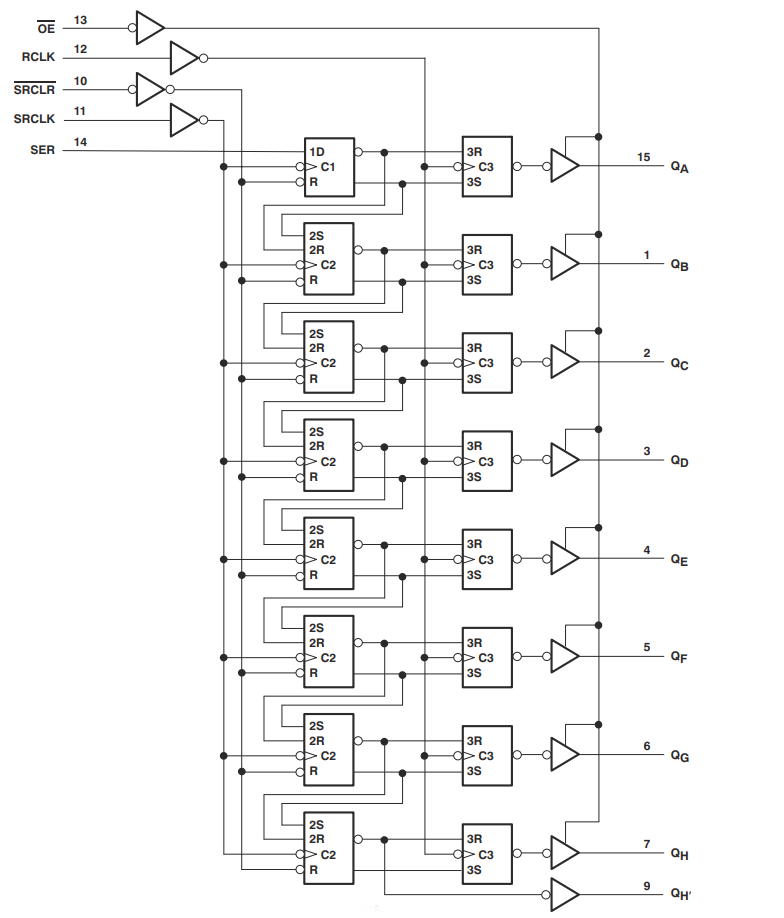
\includegraphics[width=1\textwidth]{figures/SR_blocos.png}
    \caption{Diagrama de blocos SN74HC595 \cite{SN74HC595}}
    \label{fig:SN74HC595blocos}
\end{figure}h

Na transmissão das tramas optou-se por dividir as duas: envio de 8 \textit{bits} na experiência da Lei de Ohm e envio de 13 \textit{bits} nas experiências de rectificadores e filtros. Como se pode ver na Tabela \ref{Table:funcSN74HC595}, são precisos 5 \acrshort{gpio}s (ou 5 saídas) para controlar o envio de uma trama, portanto, para realizar o comando dos relés do \acrshort{lare}, são/serão necessários 10 \acrshort{gpio}s.
Nos capítulos seguintes - \textbf{COLOCAR A REFERÊNCIA} - é explicado com mais pormenor o processo de envio. As implicações ao nível do \textit{software} de programação são mínimas e ao nível do \textit{hardware} estão dentro dos limites de número de \acrshort{gpio}s do \gls{RaspberryPI}.

\begin{table}[htb]
    \caption{Modos de funcionamento do SN74HC595 \cite{SN74HC595}}
    \label{Table:funcSN74HC595}
    \resizebox{\textwidth}{!}{%
        \begin{tabular}{cccccl}
            \toprule
            \multicolumn{5}{c}{Entradas}           & \multicolumn{1}{c}{\multirow{3}{*}{Função}}                                                                                        \\
            \cline {1-5}
            \multicolumn{5}{l}{}                   &
            \multicolumn{1}{c}{}                                                                                                                                                        \\
            \multicolumn{1}{l}{SER}                &
            \multicolumn{1}{l}{SRCLK}              &
            \multicolumn{1}{l}{$\overline{SRCLR}$} &
            \multicolumn{1}{l}{RCLK}               &
            \multicolumn{1}{l}{$\overline{OE}$}    &
            \multicolumn{1}{c}{}                                                                                                                                                        \\
            \midrule
            X                                      & X                                           & X & X          & H & Saídas $Q_A$ – $Q_H$ estão desabilitadas.                       \\
            \midrule
            X                                      & X                                           & X & X          & L & Saídas $Q_A$ – $Q_H$ estão habilitadas.                         \\
            \midrule
            X                                      & X                                           & L & X          & X & Registo de deslocamento é limpo.                                \\
            \midrule
            L                                      &
            $\uparrow$                             &
            H                                      &
            X                                      &
            X                                      &
            \begin{tabular}[c]{@{}l@{}} Primeiro passo do registo de deslocamento vai a ``0''. \\ Passo seguinte armazena os dados do estado anterior, respectivamente. \end{tabular}   \\
            \midrule
            H                                      &
            $\uparrow$                             &
            H                                      &
            X                                      &
            X                                      &
            \begin{tabular}[c]{@{}l@{}}Primeiro passo do registo de deslocamento vai a ``1''. \\ Passo seguinte armazena os dados do estado anterior, respectivamente. \end{tabular}    \\
            \midrule
            X                                      & X                                           & X & $\uparrow$ & X & Os dados do registo de deslocamento são armazenados no registo. \\
            \bottomrule
        \end{tabular}%
    }
\end{table}

\textbf{No datasheet em tal sítio está representada informação complementar respeitante ao ULN2003A e 74595}

\subsubsection{Outras coisas | Vários}
\textbf{Acho que nada tenho a referir, pelo menos que me lembre}

\section{Software}
\label{sec:software}
O \textit{software} do \acrshort{lare} foi dividido em duas grandes grupos/partes/secções(riscar o que não interessa): \textit{Back-end} e \textit{Front-end}.

Por \textit{Back-end} pode entender-se toda a programação e os processos a correr em segundo plano, que sustentam o funcionamento do \acrshort{lare}, incluindo servidor, \acrshort{api}s ou base de dados \cite{FrontbackEnd}. Existe uma grande variedade de linguagens de programação, \textit{frameworks} e ferramentas para realizar a gestão do \textit{Back-end}. Na implementação do \acrshort{lare}, utilizou-se o \textit{Python} como linguagem de programação e o \textit{Flask} como \textit{Framework}.

Já o \textit{Front-end} gere as partes dos \textit{sites} e das aplicações que os utilizadores veem e com as quais interagem para realizar determinadas tarefas. As linguagens utilizadas na implementação do \textit{Front-end} para o \acrshort{lare} foram o \acrshort{html}, \acrfull{css} e \textit{JavaScript}. Enquanto o \acrshort{html} é a ``espinha dorsal'' estrutural de um \textit{site}, o \acrshort{css} lida com a aparência personalizada que define o estilo dos elementos visuais e o JavaScript afecta a forma como os elementos da página se movimentam \cite{FrontbackEnd}.

De uma forma resumida, o desenvolvimento de \textit{Front-end} refere-se ao lado do cliente (aspeto de uma página \textit{Web}) e o desenvolvimento de \textit{Back-end} refere-se ao lado do servidor (funcionamento de uma página \textit{Web}).

\subsection{\textit{Back-End}}
\subsubsection{\textit{Python}}
A opção por esta linguagem deveu-se a uma série de factores que começaram com a vontade pessoal de desenvolver e evoluir ao nível do conhecimento em \textit{Python}. Além disso, e como já foi referido no Capítulo \textbf{VER REFERÊNCIA}, o comando e configuração do \acrshort{virtualbench} é feito através do \textit{pyVirtualBench}.

O \textit{Python} é uma linguagem poderosa e fácil de aprender. Possui estruturas de dados de alto nível eficientes e uma abordagem simples, mas eficaz à programação orientada para objectos \cite{ThePython}. Apresenta, também, uma série de vantagens que se enquadram nos objectivos do desenvolvimento e implementação do \acrshort{lare} \cite{pythonvantagens}:
\begin{itemize}
    \item Curva suave de aprendizagem;
    \item Quantidade e variedade das bibliotecas;
    \item Portabilidade;
    \item Flexibilidade;
    \item Robustez;
    \item Suporte da comunidade.
\end{itemize}

Como desvantagens há a referir que, comparado com outras linguagens, o \textit{Python} é mais lento em termos de execução, já que é um tipo de linguagem de alto-nível, não é adaptado para aplicações móveis e consome mais recursos \cite{pythonvantagens} \cite{5MainDispython}.

Ainda assim, segundo a \textit{\href{https://spectrum.ieee.org/the-top-programming-languages-2023}{\textit{IEEE Spectrum}}} o \textit{Python} foi considerada a linguagem mais popular em 2023.

\subsubsection{\textit{Flask}}
O \textit{Flask} é uma \textit{framework} leve e flexível para \textit{Python} que segue a filosofia \textit{UNIX} de ``fazer uma coisa bem feita''. A escolha do \textit{Flask} deveu-se, essencialmente, à facilidade de integração com o \textit{Python}, sendo uma das \textit{frameworks} mais populares em \textit{Python} \cite{Flask}. É uma \textit{framework} de aplicações \acrfull{wsgi} que descreve a forma como um servidor \textit{Web} comunica com aplicações \textit{Web} e como essas aplicações podem ser encadeadas para processar um pedido \cite{wsgi}. Depende, ainda do  \textit{Jinja}, que é um motor de criação de modelos que permite escrever código semelhante à sintaxe do \textit{Python}, de forma a renderizar o documento final \cite{Jinja}.

Tal como foi referido na Secção \ref{sec:contextualização}, foram ainda analisadas várias opções, incluindo a \textit{Django}, outra \textit{framework} bastante popular. Em \cite{Djangovsflask} e \cite{FlaskvsDjango}, por exemplo, é feita uma comparação exaustiva entre as duas \textit{frameworks}, não havendo uma decisão final sobre qual a melhor, mas sim sobre qual a que melhor se adapta às necessidades de implementação e desenvolvimento dos projectos.

No entanto, o \textit{Flask} foi concebido para tornar a iniciação rápida e fácil, com a capacidade de evoluir até aplicações mais complexas, sendo mais adapatado a pequenos projectos.

Pelas razões referidas anteriormente, assim como a análise feita aos prós e contras, considerou-se que tanto o \textit{Python} como o \textit{Flask} são as linguagens que melhor se enquadram e adaptam aos objectivos propostos para o \acrshort{lare}.

\subsection{Front-End}
\subsubsection{\textit{Webpage}}
Como já foi referido na Secção \ref{sec:software}, o \textit{Front-end} diz respeito ao aspecto gráfico das páginas \textit{Web} e pretende-se que a prioridade na construção da página seja a simplicidade.

A escolha do desenvolvimento da página recaiu no \acrshort{html}, \acrshort{css} e (pontualmente - \textbf{REVER}) \textit{JavaScript}.

O \acrshort{html} é a linguagem de marcação \textit{standard}, usada para definir a estrutura do seu conteúdo e consiste numa série de elementos usados para delimitar ou agrupar diferentes partes do conteúdo. As \textit{tags} podem transformar uma palavra ou imagem num \textit{hiperlink}, podem colocar palavras em itálico, podem aumentar ou diminuir a fonte, etc. etc. \cite{HTMLbasics}.

A folha de estilos \acrshort{css} é o código usado para dar estilo à página. Assim como o \acrshort{html}, o \acrshort{css} não é, realmente, uma linguagem de programação. Também não é uma linguagem de marcação — é uma linguagem de folhas de estilos. Isso significa que o \acrshort{css} permite aplicar estilos seletivamente a elementos em documentos \acrshort{html}.

Já o \textit{JavaScript} é uma linguagem de programação utilizada principalmente para \textit{scripts} dinâmicos do lado do cliente em páginas \textit{web}, podendo também ser utilizada no lado do servidor. É também utilizado no navegador, permitindo que os conteúdos das páginas sejam manipulados através de uma \acrshort{api} \acrfull{dom} ou através de \acrfull{ajax} \cite{HTMLbasics}.